\section{Empirical Performance Analysis}\label{fairness_fairXplainer_sec:experiments}
In this section, we perform an empirical evaluation of {\fairXplainer}. Particularly, we discuss the experimental setup, the objectives of experiments, and experimental results. 

\paragraph{Experimental Setup.} We implement a prototype of {\fairXplainer} in Python (version $ 3.7.6 $). To estimate FIFs, we leverage and modify the `HDMR' module in SALib library~\cite{Herman2017} based on global sensitivity analysis. In experiments, we consider four widely studied datasets from fairness literature, namely German-credit~\cite{Dua:2019},
% Ricci~\cite{mcginley2010ricci}, 
Titanic (\url{https://www.kaggle.com/c/titanic}), COMPAS~\cite{angwin2016machine}, and Adult dataset~\cite{Dua:2019}. We deploy Scikit-learn~\cite{scikit-learn} to learn different classifiers: logistic regression classifier, support vector machine (SVM), neural network, and decision tree with $ 5 $-fold cross-validation. In experiments, we specify {\fairXplainer} to compute intersectional influences up to the second order ($ \lambda = 2 $). While applying cubic-spline based local regression in {\fairXplainer}, we set $ \tau $, the number of spline intervals to $ 6 $. We compare {\fairXplainer} with the existing Shapley-valued based FIF computational framework (\url{https://shorturl.at/iqtuX}), referred as SHAP~\cite{lundberg2020explaining}. For both {\fairXplainer} and SHAP, we set a timeout of $ 300 $ seconds for estimating FIFs. In addition, we deploy {\fairXplainer} along with a fairness-enhancing algorithm~\cite{kamiran2012data} and a fairness attack~\cite{solans2020poisoning} algorithm, and analyze the effect of these algorithms on the FIFs and the resultant fairness metric. In the following, we discuss the objectives of our empirical study. 


\begin{enumerate}
%\begin{enumerate}
	\item \textit{Performance:} How \textbf{accurate and computationally efficient} {\fairXplainer} and SHAP are in approximating the bias of a classifier based on estimated FIFs?
	\item \textit{Functionality:} How do FIFs estimated by {\fairXplainer} and SHAP \textbf{correlate with the impact a fairness intervention} strategy on features?
%    \item \textit{Ablation study:} What are the effects of different \textbf{hyper-parameters} on accuracy and efficiency of {\fairXplainer}?
	\item \textit{Granularity of explanation:} How effective are the \textbf{ intersectional FIFs} in comparison with the \textbf{individual FIFs} while tracing the sources of bias?
	\item \textit{Application:} How do FIFs quantify the impact of \textbf{applying} different fairness enhancing algorithms, i.e. \textbf{affirmative actions}, and fairness attacks, i.e. \textbf{punitive actions}?
 %\item \red{What is the effect of $ \lambda $ on the runtime of {\fairXplainer}?}
\end{enumerate}

In summary, (1) we observe that {\fairXplainer} yields \textit{less estimation error} than SHAP while approximating statistical parity using FIFs. {\fairXplainer} incurs lower execution time, i.e. \textit{better efficiency in computing individual FIFs} than SHAP while also enabling computation of intersectional FIFs for real-world datasets and classifiers. (2) While considering a fairness intervention, i.e. change in bias due to omission of a feature, FIFs estimated by {\fairXplainer} have \textit{higher correlation with increase/decrease in bias due to  the intervention than SHAP}. %importantly by top most features with highest absolute FIFs. 
Thus, {\fairXplainer} demonstrates to be \textit{a better choice for identifying the features influencing the group fairness metrics} than SHAP. 
%(3) In the ablation study, {\fairXplainer} demonstrates the trade-off between estimation accuracy and execution time through hyper-parameters $ \tau $ and $ \lambda $. 
(3) \textit{By quantifying both the individual and intersectional influences of features, \fairXplainer{} leads to a more accurate and granular interpretation of the sources of bias}, which is absent in earlier bias explaining methods like SHAP. (4) Finally, as an application of the FIF formulation, {\fairXplainer} also detects the effects of the affirmative and punitive actions on the bias of a classifier and the corresponding tensions between different subsets of features.  Here, we elaborate on experimental results, and defer additional experiments such as applying {\fairXplainer} on other fairness metrics: equalized odds and predictive parity, and an ablation study of hyper-parameters: maximum order of intersectionality  $ \lambda $ and spline intervals $ \tau $ to Appendix~\ref{fairness_fairXplainer_sec:additional_experiments}.

\begin{table*}    
	\caption[Approximation error of $ \mathsf{SP} $ using FIFs]{Median error (over 5-fold cross validation and all combinations of sensitive features) of estimating statistical parity, $ |\mathsf{SP} - \widehat{\mathsf{SP}}| $, using FIFs computed by different methods (columns $ 5 $ to $ 7 $). Best results (lowest error) are in bold color. `{\textemdash}' denotes timeout.}\label{fairness_fairXplainer_tab:fair_algo_verification}  
	\small{	 
	\centering
	%        \setlength{\tabcolsep}{.3em}
	\begin{tabular}{lrclrrrr}
		\toprule
		\multirow{2}{*}{Dataset} & \multirow{2}{*}{\shortstack[1]{Dimension\\$ (n, \numfeatures) $}} & \multirow{2}{*}{\shortstack[1]{Max $ |\sensitive| $}} &\multirow{2}{*}{Classifier} & \multirow{2}{*}{SHAP} & \multicolumn{2}{c}{\fairXplainer}\\
		& & & & & $ \lambda = 1 $ & $ \lambda = 2 $\\
		\midrule
		

	
\multirow{4}{*}{Titanic} & \multirow{4}{*}{$ (834, 11) $} & \multirow{4}{*}{$ 3$} 
& Logistic Regression &  $ 2.018 $ &  $ 0.218 $ &  $ \mathbf{0.003} $ &  \\ 
& & & SVM &  $ 1.000 $ &  $ 0.137 $ &  $ \mathbf{0.000} $ &  \\ 
& & & Neural Network & \textemdash &  $ 0.215 $ &  $ \mathbf{0.003} $ &  \\ 
& & & Decision Tree &  $ \mathbf{0.018} $ &  $ 0.396 $ &  $ 0.079 $ &  \\ 
\midrule

\multirow{4}{*}{German} & \multirow{4}{*}{$ (417, 23) $} & \multirow{4}{*}{$ 2$} 
& Logistic Regression &  $ 0.361 $ &  $ \mathbf{0.205} $ & \textemdash &  \\ 
& & & SVM &  $ 0.676 $ &  $ \mathbf{0.218} $ & \textemdash &  \\ 
& & & Neural Network & \textemdash &  $ 0.181 $ &  $ \mathbf{0.001} $ &  \\ 
& & & Decision Tree &  $ \mathbf{0.000} $ &  $ 0.262 $ &  $ 0.001 $ &  \\ 
\midrule

\multirow{4}{*}{COMPAS} & \multirow{4}{*}{$ (5771, 8) $} & \multirow{4}{*}{$ 3$} 
& Logistic Regression &  $ 0.468 $ &  $ 0.118 $ &  $ \mathbf{0.056} $ &  \\ 
& & & SVM &  $ 0.360 $ &  $ 0.037 $ &  $ \mathbf{0.020} $ &  \\ 
& & & Neural Network & \textemdash &  $ 0.108 $ &  $ \mathbf{0.053} $ &  \\ 
& & & Decision Tree &  $ \mathbf{0.041} $ &  $ 0.087 $ &  $ 0.055 $ &  \\ 
\midrule

\multirow{4}{*}{Adult} & \multirow{4}{*}{$ (26048, 11) $} & \multirow{4}{*}{$ 3$} 
& Logistic Regression &  $ 2.751 $ &  $ 0.109 $ &  $ \mathbf{0.011} $ &  \\ 
& & & SVM &  $ 0.963 $ &  $ 0.095 $ &  $ \mathbf{0.001} $ &  \\ 
& & & Neural Network & \textemdash &  $ 0.067 $ &  $ \mathbf{0.000} $ &  \\ 
& & & Decision Tree &  $ \mathbf{0.027} $ &  $ 0.146 $ &  $ 0.081 $ &  \\

		\bottomrule
	\end{tabular}
}
%	\vspace*{1em}
\end{table*}



\begin{comment}






\begin{table*}       
	\centering
	%        \setlength{\tabcolsep}{.3em}
	\begin{tabular}{lrrlrrrr}
		\toprule
		Dataset & Dimension & \#Sensitive Feat. & Classifier & SHAP & \multicolumn{2}{c}{\fairXplainer}\\
		& & & & & $ \lambda = 1 $ & $ \lambda = 2 $\\
		\midrule
		
		\multirow{4}{*}{Ricci} & \multirow{4}{*}{$ (94, 5) $} & \multirow{4}{*}{$ 2$} 
		& Logistic Regression &  $ \mathbf{0.06} $ &  $ 0.19 $ &  $ 1.3 $ &  \\ 
		& & & SVM &  $ \mathbf{0.06} $ &  $ 0.19 $ &  $ 1.92 $ &  \\ 
		& & & Neural Network &  $ 2.55 $ &  $ \mathbf{0.19} $ &  $ 1.9 $ &  \\ 
		& & & Decision Tree &  $ \mathbf{0.05} $ &  $ 0.19 $ &  $ 2.23 $ &  \\ 
		\midrule
		
		\multirow{4}{*}{Titanic} & \multirow{4}{*}{$ (834, 7) $} & \multirow{4}{*}{$ 3$} 
		& Logistic Regression &  $ \mathbf{0.09} $ &  $ 0.26 $ &  $ 31.26 $ &  \\ 
		& & & SVM &  $ \mathbf{0.11} $ &  $ 0.31 $ &  $ 25.71 $ &  \\ 
		& & & Neural Network & \textemdash &  $ \mathbf{0.28} $ &  $ 22.89 $ &  \\ 
		& & & Decision Tree &  $ \mathbf{0.22} $ &  $ 0.27 $ &  $ 21.68 $ &  \\ 
		\midrule
		
		\multirow{4}{*}{COMPAS} & \multirow{4}{*}{$ (5771, 9) $} & \multirow{4}{*}{$ 3$} 
		& Logistic Regression &  $ \mathbf{0.19} $ &  $ 0.34 $ &  $ 31.64 $ &  \\ 
		& & & SVM &  $ \mathbf{1.18} $ &  $ 1.44 $ &  $ 32.68 $ &  \\ 
		& & & Neural Network & \textemdash &  $ \mathbf{0.34} $ &  $ 19.79 $ &  \\ 
		& & & Decision Tree &  $ 1.35 $ &  $ \mathbf{0.3} $ &  $ 36.58 $ &  \\ 
		\midrule
		
		\multirow{4}{*}{Adult} & \multirow{4}{*}{$ (26048, 8) $} & \multirow{4}{*}{$ 3$} 
		& Logistic Regression &  $ \mathbf{0.43} $ &  $ 0.96 $ &  $ 27.74 $ &  \\ 
		& & & SVM &  $ \mathbf{13.11} $ &  $ 15.28 $ &  $ 31.12 $ &  \\ 
		& & & Neural Network & \textemdash &  $ \mathbf{0.45} $ &  $ 25.48 $ &  \\ 
		& & & Decision Tree &  $ 13.35 $ &  $ \mathbf{0.69} $ &  $ 28.25 $ &  \\ 
		
		\bottomrule
	\end{tabular}
	\caption{Median execution time in seconds.} \label{tab:fair_algo_verification}
\end{table*}


\end{comment}


\subsection{Performance and Functionality in Estimating FIFs}
\paragraph{Accurate Approximation of Bias with FIFs.} We compare {\fairXplainer} with SHAP in estimating statistical parity by summing all FIFs, as dictated by the decomposability property (Theorem~\ref{fairness_fairXplainer_thm:fif_property}). {To our best knowledge, the ground truth of FIF is not known for real-world datasets and classifiers. As such, we cannot compare accuracy of {\fairXplainer} and SHAP directly on the estimated FIFs. Since both methods follow the decomposability property, one way to compare them is to test accuracy of the sum of estimated FIFs yielding bias/unfairness, as the ground truth of bias of a classifier can be exactly calculated for a given dataset~\cite{aif360-oct-2018}.}
We compute estimation error by taking the absolute difference between the exact and  estimated values of statistical parity, and present median results in Table~\ref{fairness_fairXplainer_tab:fair_algo_verification}. 

In general, {\fairXplainer} achieves less estimation with $ \lambda = 2 $ than with $ \lambda = 1 $ in all datasets and classifiers. This implies that combining intersectional FIFs with individual FIFs captures bias more accurately than the individual FIFs alone. In each dataset, {\fairXplainer} ($\lambda = 2$) demonstrates less estimation error than SHAP in all classifiers except in decision trees, denoting that GSA based approach {\fairXplainer} is more accurate in approximating group fairness metrics through FIFs than the local explainer SHAP. In decision trees, {\fairXplainer}\textemdash which is model-agnostic in methodology\textemdash with $ \lambda = 2 $ often demonstrates a comparable accuracy with SHAP, especially the optimized tree-based explanation counterpart of SHAP~\cite{lundberg2020local2global}. In the context of neural networks, SHAP, particularly Kernel-SHAP, often fails to estimate FIFs within the provided time-limit, while {\fairXplainer} with $ \lambda = 2 $ yields highly accurate estimates (median estimation error between $ 0$ to $0.053 $). Therefore, we conclude that \emph{{\fairXplainer} is more accurate in estimating statistical parity using FIFs than SHAP.}

\begin{figure}
	\centering
	\subfloat{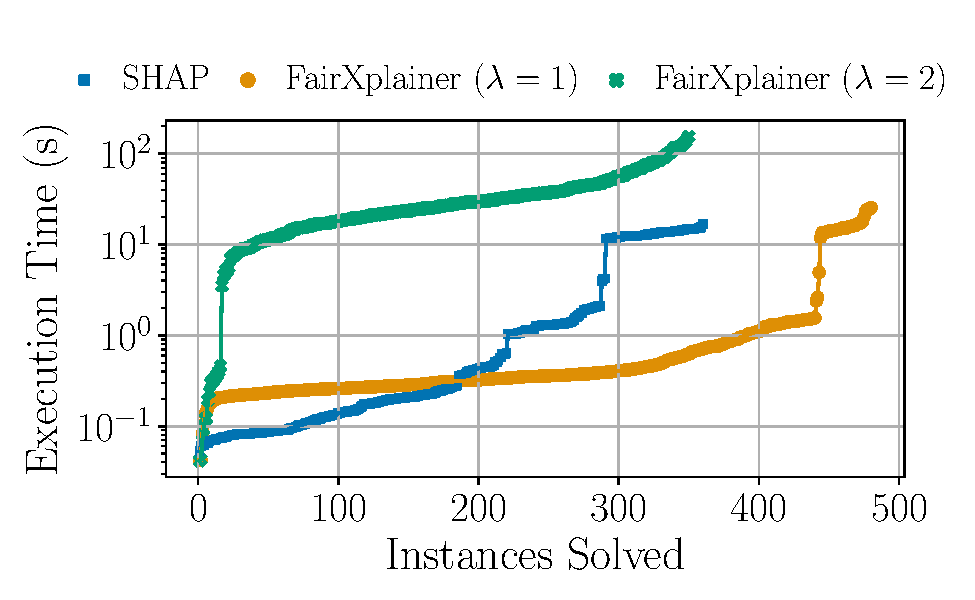
\includegraphics[scale=0.5]{figures/fairness/fif/runtime_diff_methods_train_sp}}
	\caption[Execution time of FIFs in $ \mathsf{SP} $]{Execution time of different methods for estimating FIFs. {\fairXplainer} with $ \lambda = 1 $ is more efficient than SHAP, while {\fairXplainer} ($ \lambda = 2 $) requires more computational effort.
	}
	\label{fairness_fairXplainer_fig:execution_time_cactus_plot}
\end{figure}



\paragraph{Execution Time: {\fairXplainer} vs.\ SHAP} We compare the execution time of {\fairXplainer} vs.\ SHAP in a cactus plot in Figure~\ref{fairness_fairXplainer_fig:execution_time_cactus_plot}, where a point $ (x, y) $ denotes that a method computes FIFs of $ y $ many fairness instances within $ x $ seconds. We consider $ 480 $ fairness instances from $ 4 $ datasets constituting $ 24 $ distinct combinations of sensitive features, $ 4 $ classifiers, and $ 5 $ cross-validation folds. In Figure~\ref{fairness_fairXplainer_fig:execution_time_cactus_plot},  {\fairXplainer} with $ \lambda = 1 $ is faster than  $ \lambda = 2 $. For example, within $ 10 $ seconds, {\fairXplainer} with $ \lambda = 1 $ solves $ 443 $ instances vs.\ $ 41 $ instances with $ \lambda = 2 $.  In addition, {\fairXplainer} with $ \lambda = 1 $ solves all $ 480 $ instances compared to $ 360 $ instances solved by SHAP. Thus, {\fairXplainer} with $ \lambda = 1 $ demonstrates its higher efficiency in estimating individual FIFs compared to SHAP. While estimating intersectional FIFs, {\fairXplainer} also demonstrates its practical applicability by solving $ 350 $ instances within  $ 160 $ seconds. \textit{Therefore, {\fairXplainer} demonstrates computational efficiency in explaining group fairness metrics of real-world datasets and classifiers.}


\begin{figure}
	\centering
	\subfloat[COMPAS]{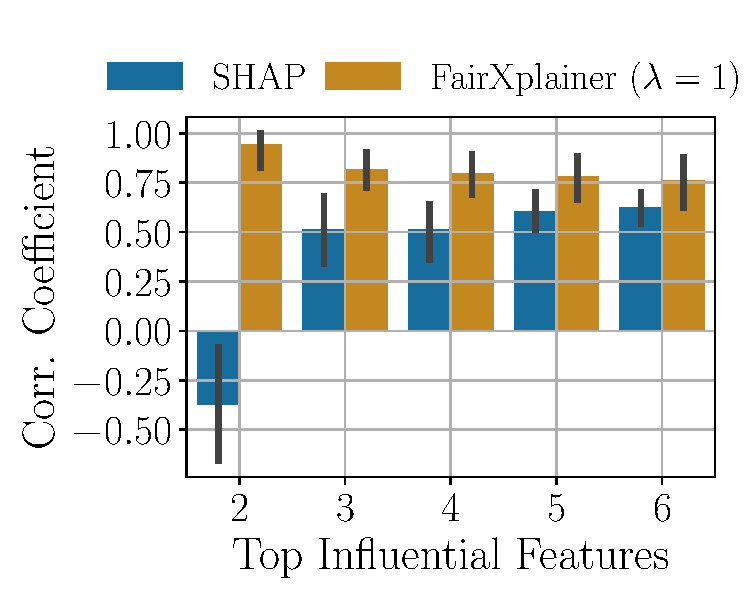
\includegraphics[scale=0.5]{figures/fairness/fif/intervention_compas}}
	\subfloat[Adult]{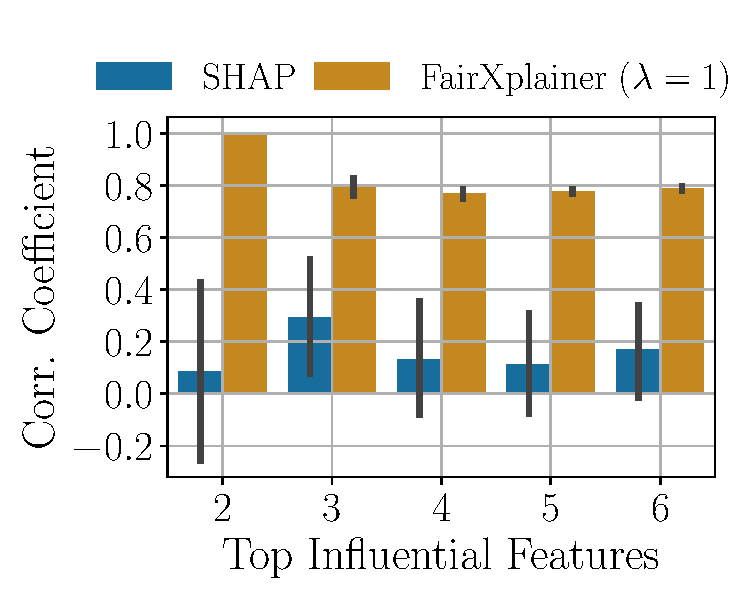
\includegraphics[scale=0.5]{figures/fairness/fif/intervention_adult}}\vspace*{-1em}
	\caption[FIFs under fairness intervention]{Results on fairness intervention on logistic regression classifiers for COMPAS and Adult datasets. Pearson's correlation coefficient between bias-difference due to the intervention and FIFs is higher for top ranked influential features by {\fairXplainer} compared to SHAP.}	
	\label{fairness_fairXplainer_fig:fairness_intervention}
\end{figure}



\paragraph{FIFs under Fairness Intervention} We consider a fairness intervention strategy to hide the impact of an individual feature on a classifier and record the correlation between fairness improvement/reduction of the intervened classifier with the FIF of the feature. Our intervention strategy of modifying the classifier is different than~\cite{datta2016algorithmic}, where the dataset is modified by replacing features with random values. In particular, we intervene a logistic regression classifier by setting the coefficient to zero for the corresponding feature. Intuitively, when the coefficient becomes zero for a feature, the prediction of the classifier may become independent on the feature; thereby, the bias of the classifier may also be independent on the conditional variances of the feature for different sensitive groups.  As a result, a feature with a positive FIF value (i.e. increases bias) is likely to decrease bias under the intervention, and vice versa. In Figure~\ref{fairness_fairXplainer_fig:fairness_intervention}, we report Pearson's correlation coefficient between the difference in bias (statistical parity) due to intervention and the FIFs of features in COMPAS and Adult datasets, where features are sorted in descending order of their absolute FIFs estimated by {\fairXplainer} and SHAP. In {\fairXplainer}, the correlation coefficient generally decreases with an increase of top influential features, denoting that features with higher absolute FIFs highly correlate with bias-differences. SHAP, in contrast, demonstrates less correlation, specially for the top most influential features. \emph{Therefore, FIFs estimated by {\fairXplainer} shows the potential of being deployed to design improved fairness algorithms in future.}



























\begin{figure}
	\centering
	\subfloat[{\fairXplainer} ($ \lambda = 1 $)]{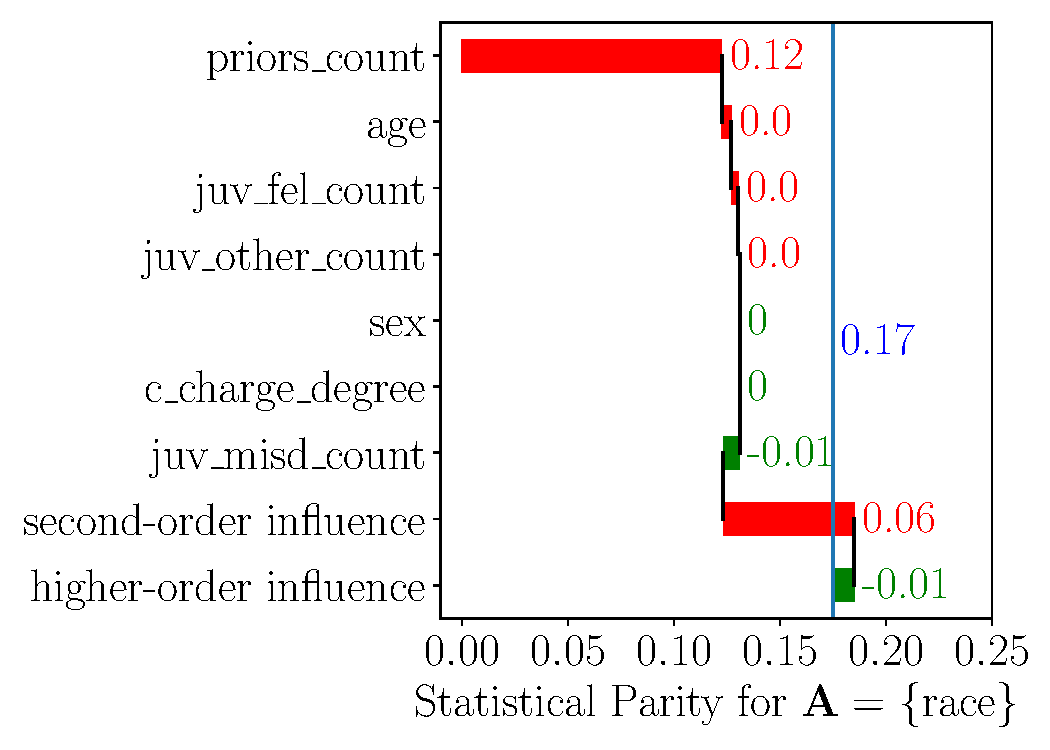
\includegraphics[scale=0.45]{figures/fairness/fif/feature_weight_unsorted}\label{fairness_fairXplainer_fig:individual_fifs}}\hfil
	\subfloat[{\fairXplainer} ($ \lambda = 2 $)]{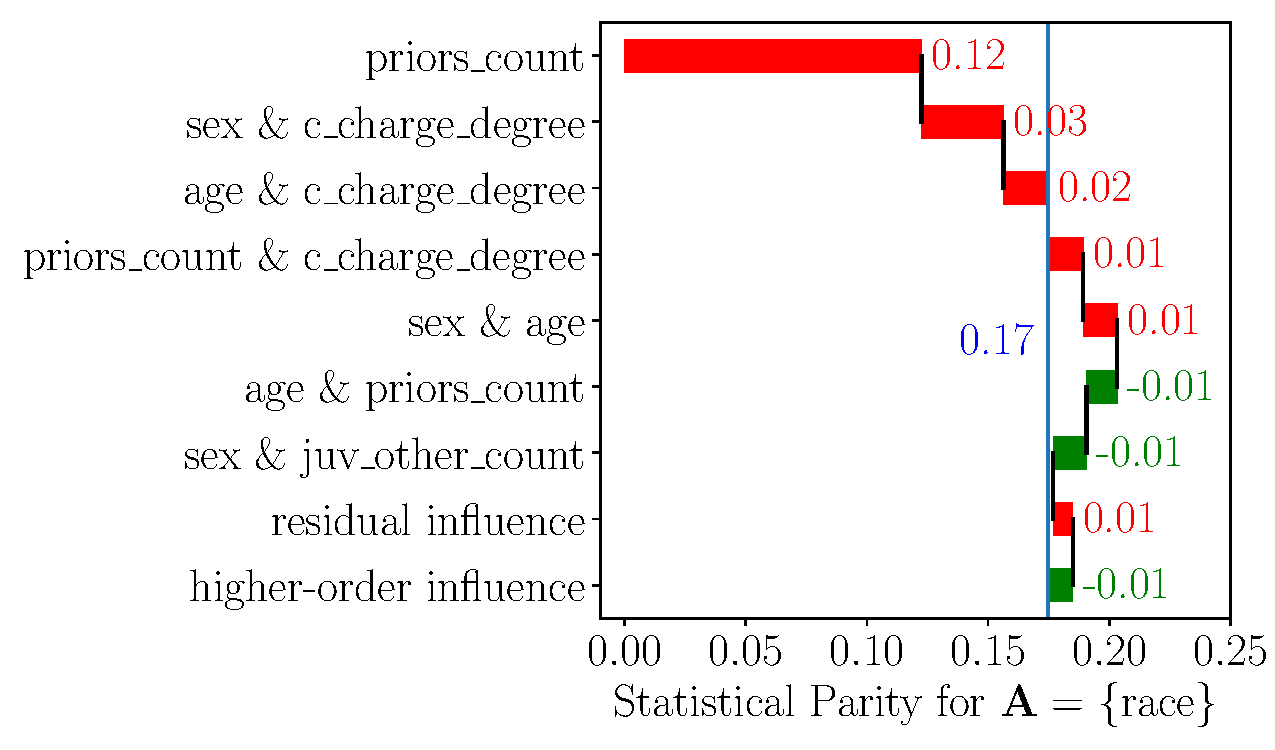
\includegraphics[scale=0.45]{figures/fairness/fif/feature_weight}\label{fairness_fairXplainer_fig:intersectional_fifs}}\hfil
	\subfloat[SHAP]{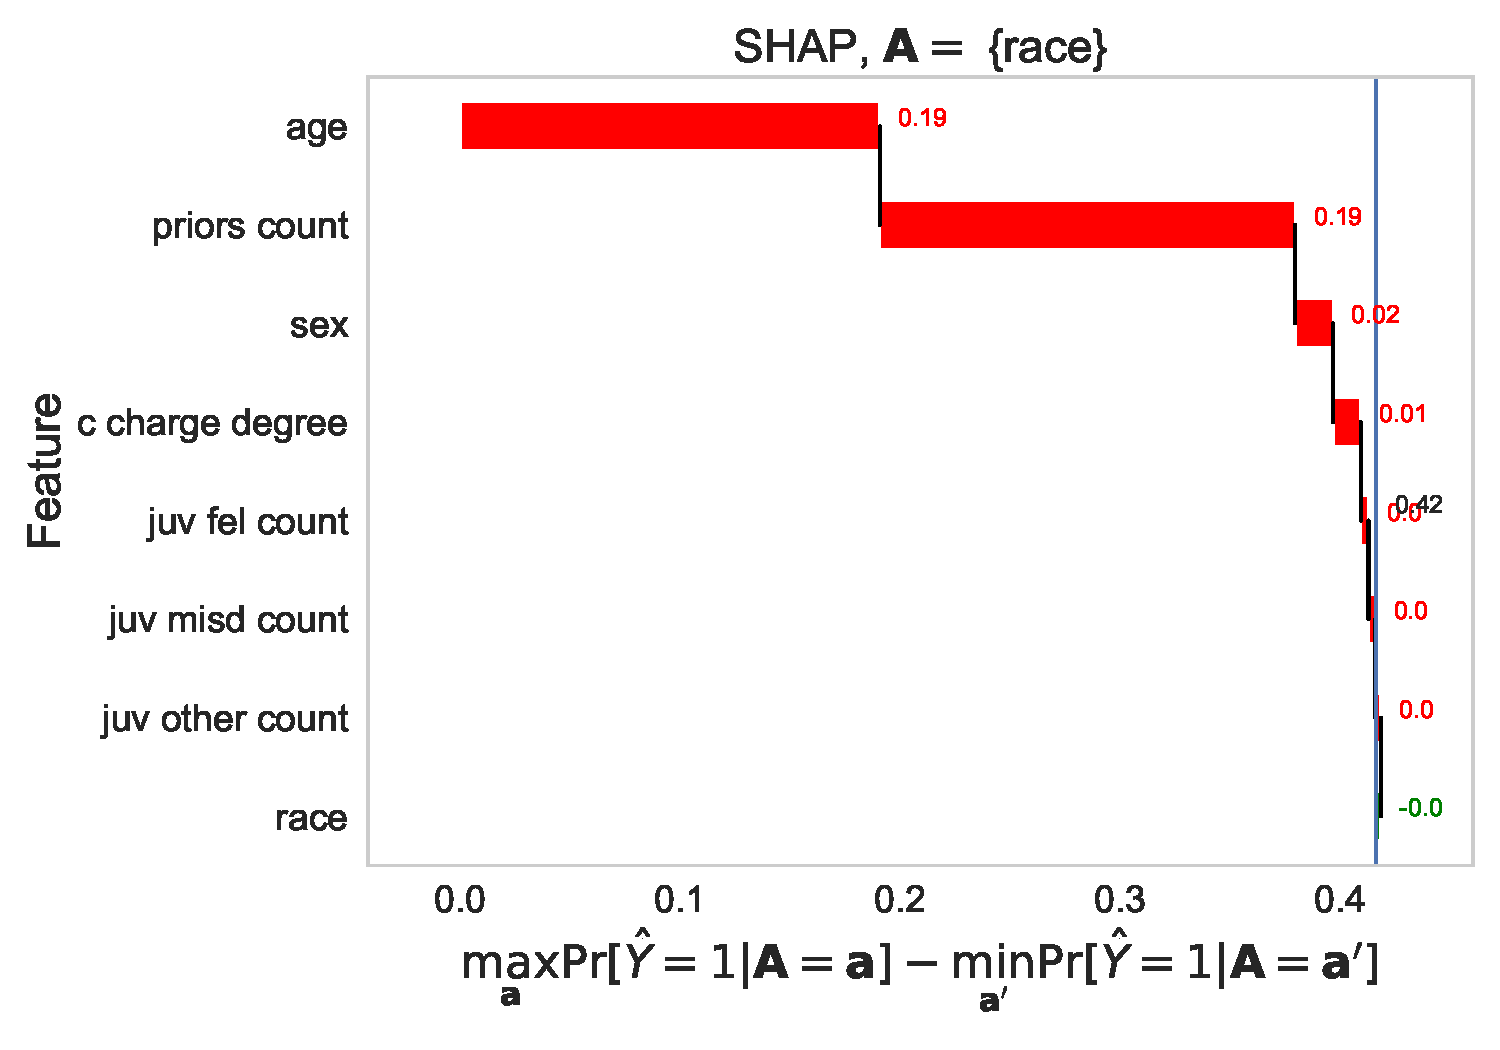
\includegraphics[scale=0.45]{figures/fairness/fif/feature_weight_shap}\label{fairness_fairXplainer_fig:fif_shap}}
	
	\caption[FIFs for COMPAS dataset]{FIFs for COMPAS dataset on explaining statistical parity. Both individual and intersectional FIFs in Figure~\ref{fairness_fairXplainer_fig:intersectional_fifs} depict sources of bias in detail than individual FIFs alone in Figure~\ref{fairness_fairXplainer_fig:individual_fifs}. In Figure~\ref{fairness_fairXplainer_fig:fif_shap}, individual FIFs estimated by SHAP are far from correctly approximating statistical parity (exact value $0.174 $).}
	\label{fairness_fairXplainer_fig:fif_illustration_compas}
\end{figure}



\subsection{Explainability and Applicability of FIFs}
\paragraph{Individual vs.\ Intersectional FIFs.} Now, we aim to understand the importance of intersectional FIFs over individual FIFs in Figure~\ref{fairness_fairXplainer_fig:fif_illustration_compas}. We consider COMPAS dataset with race $ \in $ \{Caucasian, non-Caucasian\} as the sensitive feature, and a logistic regression classifier to predict whether a person will re-offend crimes within the next two years. Since the classifier only optimizes training error, it demonstrates statistical parity of $ 0.174 $, i.e. it suggests that a non-Caucasian  has $ 0.174 $ higher probability of re-offending crimes than a Caucasian. Next, we investigate the sources of bias and present individual FIFs in Figure~\ref{fairness_fairXplainer_fig:individual_fifs}, and both individual and intersectional FIFs in Figure~\ref{fairness_fairXplainer_fig:intersectional_fifs}. In both figures, we present influential features and their FIFs in the descending order of absolute values. According to {\fairXplainer}, the priors count (FIF $ = 0.1 $) dominates in increasing statistical parity\textemdash between Caucasian and non-Caucasian, their prior count demonstrates the maximum difference in the scaled variance of positive prediction. Other non-sensitive features have almost zero FIFs. However, in Figure~\ref{fairness_fairXplainer_fig:individual_fifs}, higher-order FIFs ($ \lambda > 1 $) increases statistical parity by $ 0.031 $, denoting that the data is correlated and presenting only individual FIFs is not sufficient for understanding the sources of bias. For example, while both sex and age individually demonstrate almost zero influence on bias (Figure~\ref{fairness_fairXplainer_fig:individual_fifs}), their combined effect and intersectional effects with c-charge degree, priors count, and juvenile miscellaneous count contribute highly on statistical parity. In contrast to {\fairXplainer}, SHAP only estimates individual FIFs  (Figure~\ref{fairness_fairXplainer_fig:fif_shap}) and approximates statistical parity with higher error than {\fairXplainer}.  Interestingly, {\fairXplainer} yields FIF estimates of the classifier trained on COMPAS dataset that significantly matches with the rule-based classifier extracted from the COMPAS dataset using Certifiably Optimal Rule Lists (CORELS) algorithm~\cite[Figure 3]{rudin2019stop}. From Figure 3 in~\cite{rudin2019stop}, we observe that prior count is the only feature used individually to predict arrests, while age is paired with sex and prior counts respectively. While considering second-order intersectionality, {\fairXplainer} ($ \lambda = 2 $) yields priors count, (sex, age), and (age, priors count) as \emph{three of the top four features} that explains the observation of~\cite{rudin2019stop} better than SHAP and {\fairXplainer} ($ \lambda = 1 $) considering only individual features. \emph{Therefore, {\fairXplainer} demonstrates a clearer understanding on the sources of bias of a classifier by simultaneously quantifying on intersectional influences and individual influences }.  %\todo{For a linear classifier with independent features, see if coefficient and FIFs are related.}



\begin{figure}
	\subfloat[Fairness attack (punitive actions)]{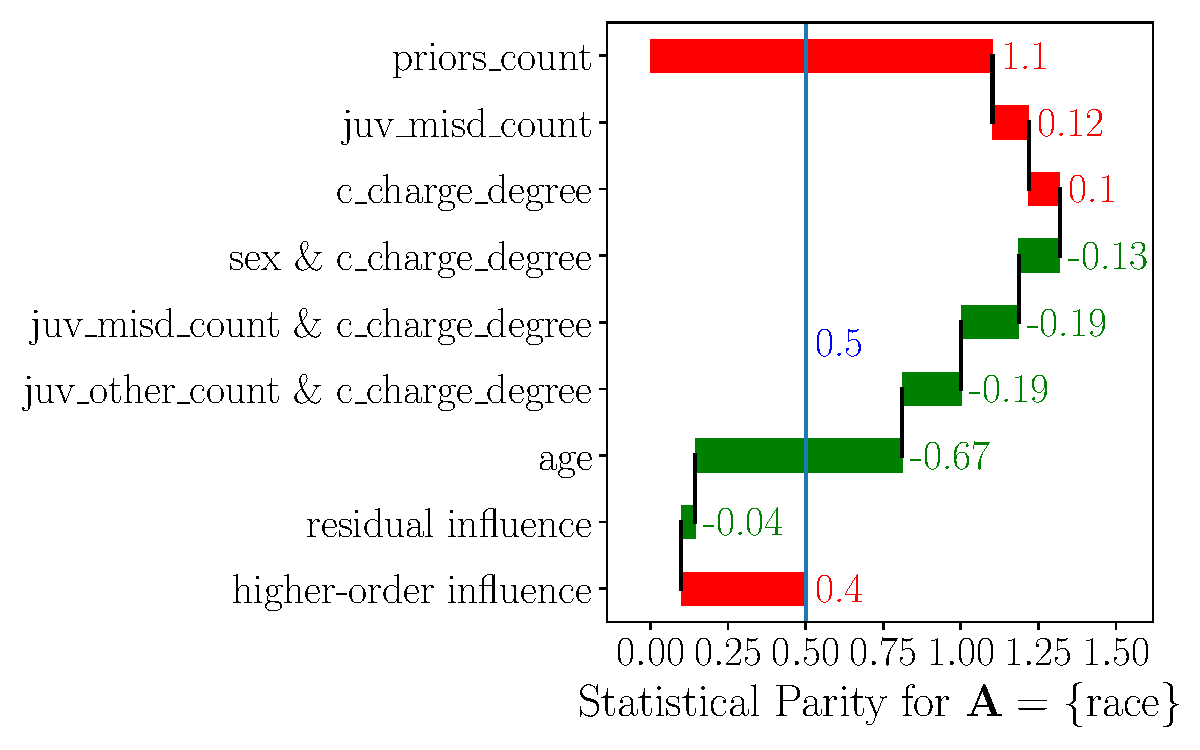
\includegraphics[scale=0.4]{figures/fairness/fif/fairness_attack}\label{fairness_fairXplainer_fig:fairness_attack}}\hfil
	\subfloat[Fairness enchancing (affirmative actions)]{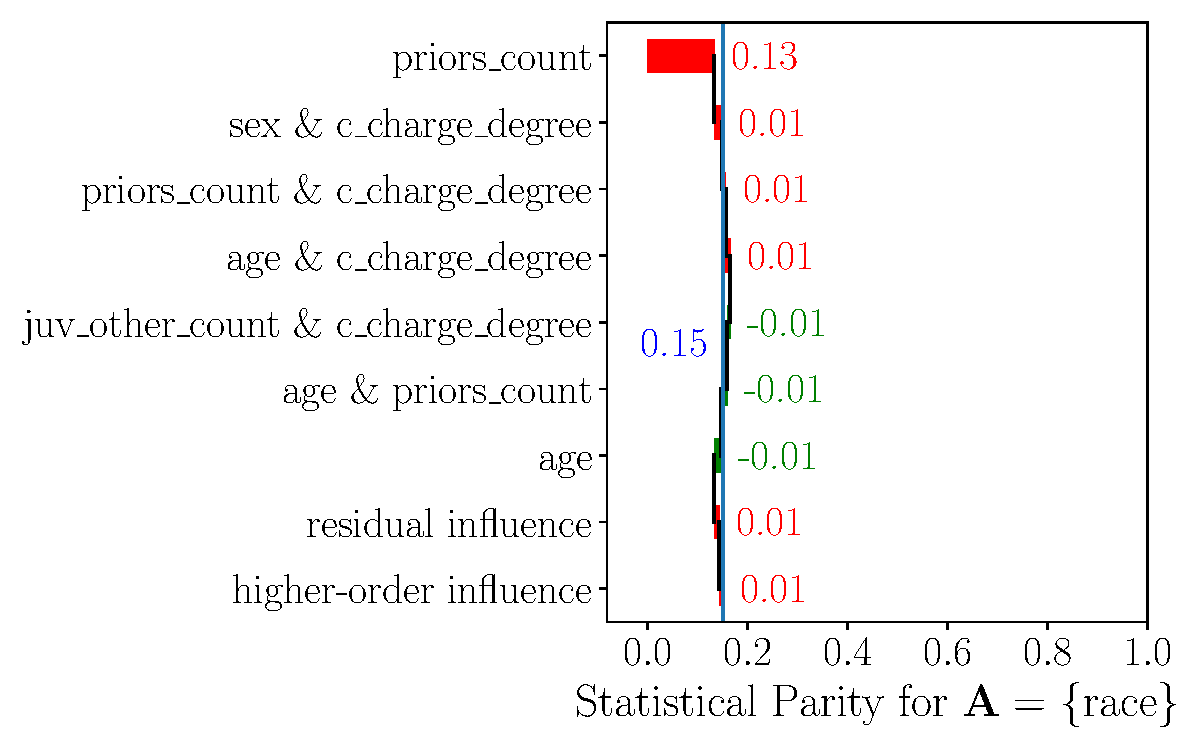
\includegraphics[scale=0.4]{figures/fairness/fif/fairness_repair}\label{fairness_fairXplainer_fig:fairness_repair}}
	
	\caption[FIFs under fairness affirmative/punitive actions]{Effects of a fairness attack~\cite{solans2020poisoning} and a fairness enhancing~\cite{kamiran2012data} algorithms on FIFs.}\label{fairness_fairXplainer_fig:affirmative_punitive_actions}
\end{figure}

\paragraph{Quantifying Impacts of Affirmative/Punitive Actions.} Continuing on the experiment in Figure~\ref{fairness_fairXplainer_fig:fif_illustration_compas}, we evaluate the effect of fairness attack and enhancing algorithms on FIFs on COMPAS dataset in Figure~\ref{fairness_fairXplainer_fig:affirmative_punitive_actions}.  Without applying any fairness algorithm, the statistical parity of the classifier is $ 0.174 $. Applying a data poisoning fairness attack~\cite{solans2020poisoning} increases statistical parity to $ 0.502 $ (approximated as $ 0.418 $ in Figure~\ref{fairness_fairXplainer_fig:fairness_attack}), whereas  a fairness-enhancing algorithm based on data reweighing~\cite{kamiran2012data} decreases statistical parity to $ 0.151 $ (approximated as $ 0.135 $ in Figure~\ref{fairness_fairXplainer_fig:fairness_repair}). In Figure~\ref{fairness_fairXplainer_fig:fairness_attack}, the attack algorithm would be more successful if it could hide the influence of features with positive FIFs, such as priors count and the intersectional effects of age and c-charge degree with sex. In contrast, in Figure~\ref{fairness_fairXplainer_fig:fairness_repair}, the fairness enhancing algorithm can improve by  further ameliorating the effect features with  negative FIFs, such as priors count. Thus, \textit{{\fairXplainer} demonstrates the potential as a dissecting tool to undertake necessary steps to improve or worsen fairness of a classifier.}





